%\documentclass{ctexart}
\documentclass{article}
\usepackage{ctex}       %载入中文包
\usepackage{graphicx}
\usepackage{eso-pic}  %水印
\usepackage{xcolor}
\AddToShipoutPictureBG{\AtPageCenter{%
  $\vcenter{%
    \makebox[0pt]{%
      \rotatebox[origin=c]{60}{%
        \scalebox{20}{%
          \bfseries\sffamily
          \color{black!60!cyan!20}%
          qjkobe%
    }}}%
  }$%
}}
\usepackage{amsmath}
%\usepackage{hyperref}
\begin{document}
\section{BN}
\subsection{What is BN?}
BN所做十分简单,即将某一层输出归一化,使得其均值为0方差为1。值得注意的是BN是在channel维度做的,即将每个channel都进行归一化,如果有n个channel那么便会有n个归一化操作。具体来说如果某个层的输出为$x=(x^{0},x^{1},...x^{n})$,那么BN 做的便是:
$$
x^{k}=\frac{x^{k}-E[x^{k}]}{\sqrt{Var[x^{k}]}}
$$

\subsection{Why need to use BN?}
BN本质上解决的是反向传播过程中的梯度问题。根据我上次所讲的反向传播,反向传播经过某层的梯度的时候,是要乘以那一层的参数的。简单回顾一下(由于是回顾,我们先忽略sigmoid),前向传播有:
$$h_l = w_l^Th_{l-1}$$
那么反向传播时便有:
$$\frac{\partial l}{\partial h_{l-1}} = \frac{\partial l}{\partial h_l} . \frac{\partial h_l}{\partial h_{l-1}} = \frac{\partial l}{\partial h_l} w_l$$
如果是从l层往k层传的话,有:
$$\frac{\partial l}{\partial h_k} = \frac{\partial l}{\partial h_l} \prod_{i=k+1}^{l} w_i
$$
上式的$\prod_{i=k+1}^l w_i$就是问题所在。因为网络层比较深,如果$w_{i}$大多小于1,那么传到很前面的时候,梯度会变得很小(梯度消失),比如$0.9^{100}$;而如果$w_{i}$大多大于1,那么传到这里的时候,梯度又会非常大(梯度爆炸),比如$1.1^{100}$。BN在做的就是解决这个问题,因为BN去除了w的scale(我的理解是尺度,大家可以根据下述理解一下)的影响。当我们做了BN 以后,有下式:
$$BN(wu)=BN((\alpha w)u)$$
$\alpha$是任意实数,这也就说明BN与w的scale是没有关系的。那么反向传播的时候,就有:
$$
\frac{\partial h_l}{\partial h_{l-1}}=\frac{\partial BN w_lh_{l-1}}{\partial h_{l-1}} =\frac{\partial BN \alpha w_lh_{l-1}}{\partial h_{l-1}}
$$
这也就是说,反向传播乘以的那个数不再和$\omega$的scale有关。进一步求梯度:
$$
\frac{\partial h_l}{\partial w_l} = \frac{\partial BNw_lh_{l-1}}{\partial w_l} = \frac{1}{\alpha}.\frac{\partial BN \alpha w_l h_{l-1}}{\partial \alpha w_l} =  \frac{1}{\alpha}.\frac{\partial BN w_l h_{l-1}}{\partial w_l}
$$
也就是说,尺度大的$\omega$会获得一个较小的梯度,每次更新会更少,这样整体的更新,就会更加稳健。

\subsection{Some extra process on BN}
\begin{figure}
  \centering
  % Requires \usepackage{graphicx}
  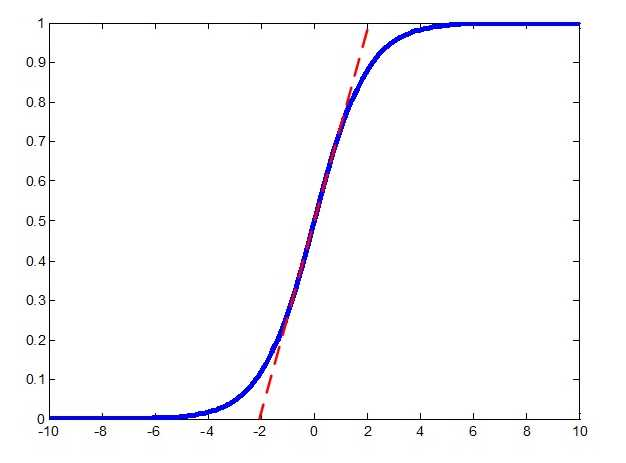
\includegraphics[width=10cm]{sigmoid}\\
  \caption{sigmoid}\label{fig:1}
\end{figure}
但是那篇论文里,不是这么简单的对BN进行操作,因为如果按照上述那种简单操作,得到的x的绝对值会特别小,会导致数据都集中在sigmoid的中间区域,如图\eqref{fig:1}所示,而这个区域是接近线性的,所以作者为了解决这个问题,就加了一个反变换:
$$
y^{(k)}=\gamma^{(k)}\widehat{x}+\beta^{(k)}
$$
而这里的两个参数,是需要学习的。作者做了一个简化,因为理想情况下,BN用到的方差和均值,应该都是针对整个数据集的,作者把它拆成了一个个mini-batch,BN转换如下:\\
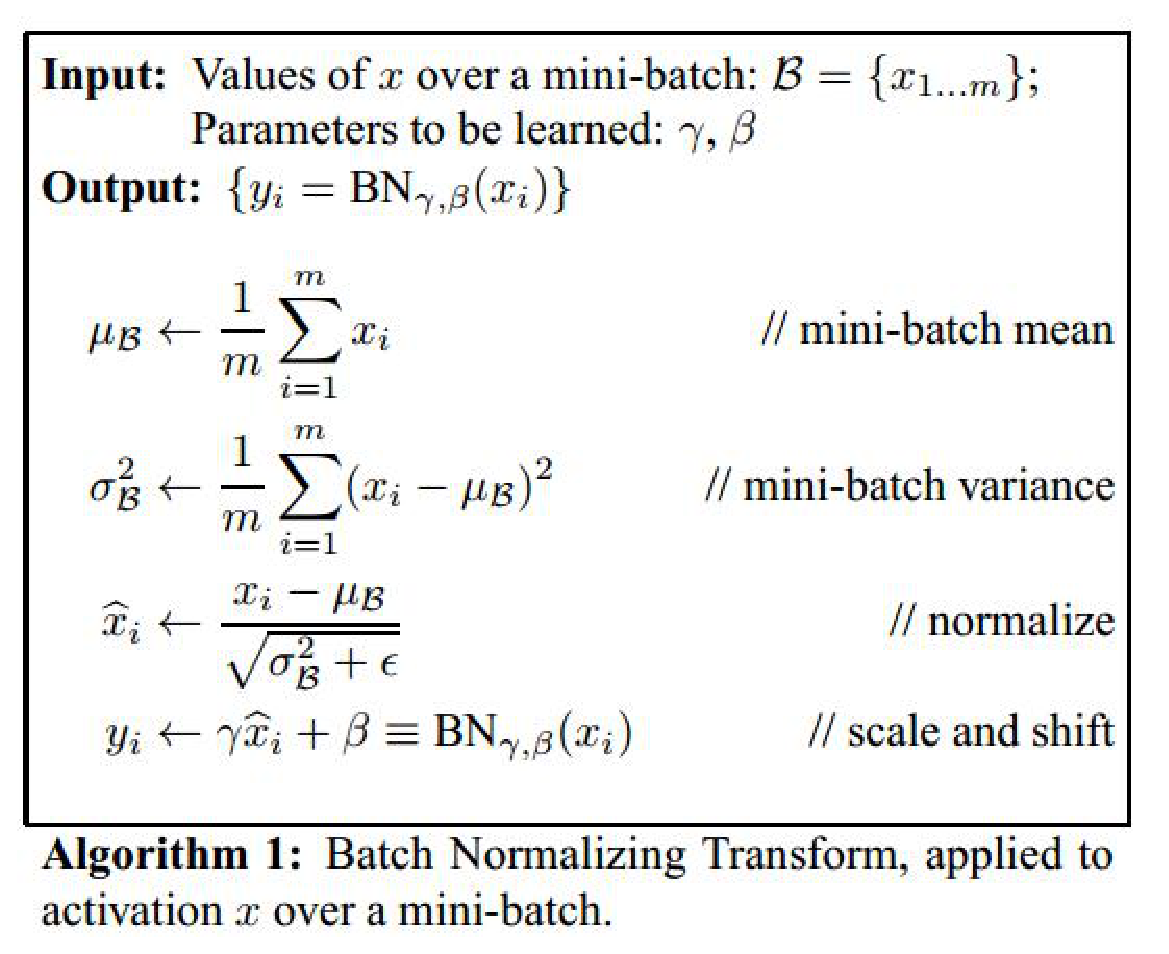
\includegraphics[width=10cm]{BN}
\\$\epsilon$是为了防止数值问题而加的一个小数,比如$10^{-6}$。(这里不太明白)。然后应用BP进行训练的时候,依旧是链式法则,这里给出各项链式的推导(对$x_{i}$做了变换,所以这里也要求对应偏导,让误差向后传播):\\
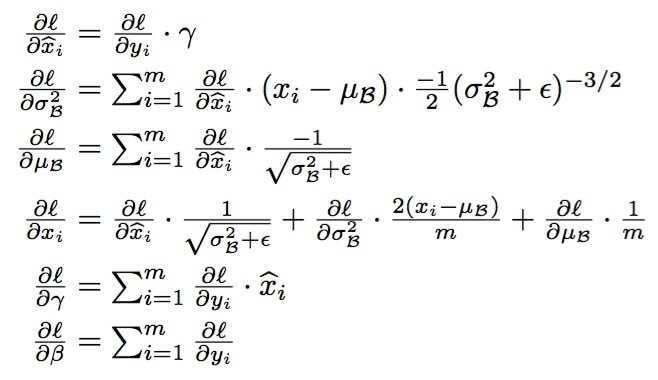
\includegraphics[width=10cm]{chain}\\
在训练最后一个mini-batch的时候,要对之前所有的mini-batch在一起求个均值,因为到时候真的有测试数据进来的话,归一化操作用的是所有训练样本中的方差和均值。
$$
E[x] \leftarrow E_{\beta}[\mu_{\beta}]
Var[x] \leftarrow \frac{m}{m-1}E_{\beta}[\sigma^{2}_{\beta}]
$$
注意这里用了m-1,也就是无偏估计(就是以前那个标准差会是样本数-1,理由不赘述)。

\subsection{BN in CNN}
这里简单说一下CNN的BN操作,因为卷积层会输出几个特征图,每个特征图都有很多神经元,如果采用BN,就会有巨多的$\gamma$和$\beta$参数,那样就太恐怖了。所以在卷积层上用BN,类似权值共享,整个特征图共享同一对参数。


\section{weight decay and momentum}
\subsection{weight decay}
在实际应用中,为了避免网络的过拟合,必须对Cost function加入一些正则项,在SGD中加入$\eta \lambda \omega _{i}$ 这一正则项对这个Cost function进行规范化:
$$
\omega_{i}\leftarrow  \omega_{i} - \eta \frac{\partial E}{\partial \omega_{i}} - \eta \lambda \omega _{i}
$$
上面这个公式基本思想就是减小不重要的参数对最后结果的影响,网络中有用的权重则不会收到Weight decay影响。

在机器学习或者模式识别中,会出现overfitting,而当网络逐渐overfitting时网络权值逐渐变大,因此,为了避免出现overfitting,会给误差函数添加一个惩罚项,常用的惩罚项是所有权重的平方乘以一个衰减常量之和(这里的衰减常量不太理解)。其用来惩罚大的权值。

\subsection{momentum}
momentum是梯度下降法中一种常用的加速技术。对于一般的SGD,其表达式为$x \leftarrow  x-\alpha \ast dx$,$x$沿负梯度方向下降。而带momentum项的SGD则写生如下形式:
$$
v=\beta \ast v -a\ast dx\\
x \leftarrow  x+v
$$
其中$\beta$ 即momentum系数,通俗的理解上面式子就是,如果上一次的momentum(即$v$)与这一次的负梯度方向是相同的,那这次下降的幅度就会加大,所以这样做能够达到加速收敛的过程。


\section{Data augmentation}
因为数据集很多时候是不够的,这样就容易导致过拟合,并且网络会很小,所以就需要一些数据增益方法:

\subsection{generating image translations and horizontal reflections}
首先将图片统一缩放到256*256大小,然后从中提取224*224的块,这样就有(256-224)*(256-224)=1024个图片,还没有结束,这1024张图片的水平镜像的图片也可以用来训练,这样就把原来一张图片变为了2048张图片。

当然这些图片都不是相互独立的,不过也可以从一定程度上解决过拟合的问题。在测试的时候,就只提取10张图片,四个角以及中心的224*224的图片和这些图片的水平镜像图片,然后对这些图片进行综合性分析。

当然这些图片都不是相互独立的,不过也可以从一定程度上解决过拟合的问题。在测试的时候,就只提取10张图片,四个角以及中心的224*224的图片和这些图片的水平镜像图片,然后对这些图片进行综合性分析。

\subsection{altering the intensities of the RGB channels in training images.}
我感觉就是,相当于同一张图片,光照条件不一样,图片是不会有变化的。原文中对RGB进行了特征分解,然后让特征值去乘以一个随机倍数,靠这个方法去得到不同的样本。

\subsection{Dropout}
这个也是防止过拟合的一种方法,简单而言就是按一定概率丢弃一部分神经元,文中不采用这个方法,只是提到了,这部分的具体知识以后再补充。
\end{document}